%************************************************
\chapter{Results}
\label{chp:results}
%\minitoc\mtcskip
%************************************************

\section{Experimental setup}
\label{sec:computationtime}
\subsection{Training material}
\label{sec:trainingmaterial}
For the unsupervised learning phase, we need a maximally large
corpus. We chose the TLG CD-ROM E, which contains about 9.3M words, and
the Perseus texts, which contain about 7.7M words. Since both corpora
share material, duplicate sentences were scrapped. The final corpus
contains about 16.9M words.

This corpus was split sentence-wise into a training corpus, from which
representations are learned, and a validation corpus, to check the
accuracy of the generated representations. The file is split 90-10.

The supervised learning phase makes use of the PROIEL annotated texts
of Herodotus and the New Testament for both morphology and
syntax. This contains approx. 195K words. Again, a validation set is
withheld, in a slightly lower proportion than in the unsupervised
phase due to the restricted size of the corpus.
\subsection{Execution}
\label{sec:execution}
For the training hyperparameters, we chose to set embedding sizes at
50. The text window size was set at 11 due to the prevalence of
long-range dependencies in ancient Greek. The learning rates for the
neural network parameters and the embeddings were set at $1.1 \cdot
10^{-8}$ and $3.4 \cdot 10^{-11}$, respectively, for the unsupervised
phase. For the supervised phase, we raised the parameter learning rate
to $0.01$. The input layer size was set equal to the window size; the
output layer size was set to 1; the hidden layer size was set to 100.

Corpus preprocessing was done on the author's own computer. We then
conducted training on an Amazon EC2 compute-optimized instance. The
unsupervised algorithm was left to generate embeddings for three days.
This was equivalent to about thirteen training epochs. The supervised
algorithm was left to iterate over the annotated corpus, finishing in
about fifteen minutes. Logs of the training process were generated,
which we converted into graphs which are displayed on the following
pages. We did not tag the corpus for reasons detailed in
\ref{chp:assessment}. The resulting language model was then serialised
for immediate reuse; a dump of the model parameters was also created
in HDF5 format.
\section{Performance}
\label{sec:performance}
\subsection{Unsupervised model}
\label{sec:unsupacc}
To quickly get a general picture of the quality of the embeddings, we
pick ten words throughout the lookup table and take their ten nearest
neighbors in the vector space according to the Euclidean metric. The
results are visible in \ref{table:nneighbors}.

The training evolution is visible from figure \ref{fig:training_loss}
onward. The red vertical lines on each graph indicate the start of new training epochs.

% We then validate the model by computing rankings for a select set of
% windows using a simple heuristic: we generate text windows from the
% validation corpus, to which we let the model assign a score. For each
% window, we generate a score for each possible corrupted version of the
% window (i.e. we replace the central word index by all other word
% indexes iteratively). The ranking of the word corresponds to the
% amount of corrupt windows which receive a higher score than the
% original window. We then compute the mean and standard deviation of
% the logarithms of these rankings.

\begin{table}
    \begin{tabular}{c|c|c|c}
\Greekσωφρόνως          & \Greekθαλαττίου     & \Greekπεριβάλλοντες & \Greekμέμψαιτο       \\
6823                    & 52759               & 67631               & 32325                \\ \hline
\Greekτ?                & \Greekατθυε         & \Greekἀποδείξειν    & \Greekἐκπορίζειν     \\
\Greekδρουγγαρίου :b co & \Greekκάμψαι        & \Greekἰέναι         & \Greekτοῖαι          \\
\Greekκτώμενοι          & \Greekκεῖνται       & \Greekἀφῃρημένον    & \Greekνημερτέα       \\
\Greekποιεῖσθε          & \GreekΣαυνίτας      & \GreekΕἵλωτας       & \Greekκτίσει         \\
\Greekδιανέμεσθαι       & \Greekἀγανακτοῦντος & \Greekἀπήνεγκαν     & \Greekκαθεστῶτα      \\
\Greekδημιουργοῦ        & \Greekπράξεως       & \Greekμυίας         & \Greekχάριτες        \\
\Greekδέρρεις           & \Greekπόλεως        & \Greekτοπικὰ        & \Greekκατηγορουμένων \\
\Greekπλανηθέντες       & \Greekπληθυντικῶς   & \Greekπελαγίαν      & \GreekΚάλλιστον      \\
\Greekπαρελάμβανεν      & \Greekταράσσειν     & \GreekΜαγδαληνὴ     & \Greekσυμπλεκομένους \\ \hline \hline
\Greekπροαιρουμένου     & \Greekἔρχεσθαι      & \Greekψεύστας       & \Greek<Περὶ          \\
96784                   & 9084                & 99698               & 6334                 \\ \hline
\Greekθυιππε            & \Greekἐρωτᾶται      & \Greekἀφελόμενος    & \Greekκεῖσε          \\
\Greekἀγνοεῖν           & \Greekἱππικὰ        & \Greekκἄλλως        & \Greekἀναλύειν       \\
\GreekΤηλεβόας          & \GreekἈθηναῖοσὦ     & \Greek<οὐχ          & \Greekσύγκρασιν      \\
\GreekἍλυς              & \Greekἑωυτῇ         & \GreekἈχελῷος       & \Greekμύραιναν       \\
\Greekεὐδοκήσας         & \Greekθαυμαστός     & \Greekδαῖμον        & \GreekΠαῦλος         \\
\Greekταλαιπωρίαις      & \Greekκαρτερὰ       & \Greekἐπανιόντα     & \Greekπαλαιστής      \\
\Greekὡρισμένος         & \Greekἥττοσι        & \Greekἐγγυᾶται      & \Greekμετάληψιν      \\
\Greekκαθεστῶτι         & \Greekκρᾶτ'         & \Greekποκ'          & \Greekφαύλῳ          \\
\Greekκαθέδρας          & \GreekΛήδας         & \Greekδιασαφῶν      & \Greekἀπετάξατο      \\
\Latin
    \end{tabular}
\caption{Eight randomly chosen words and their nearest neighbors. We
only picked words from the first 100.000 embeddings, as the cost of
computing the nearest neighbors of a point increases exponentially
when the point set becomes larger.} \label{table:nneighbors}
\end{table}

\begin{figure}
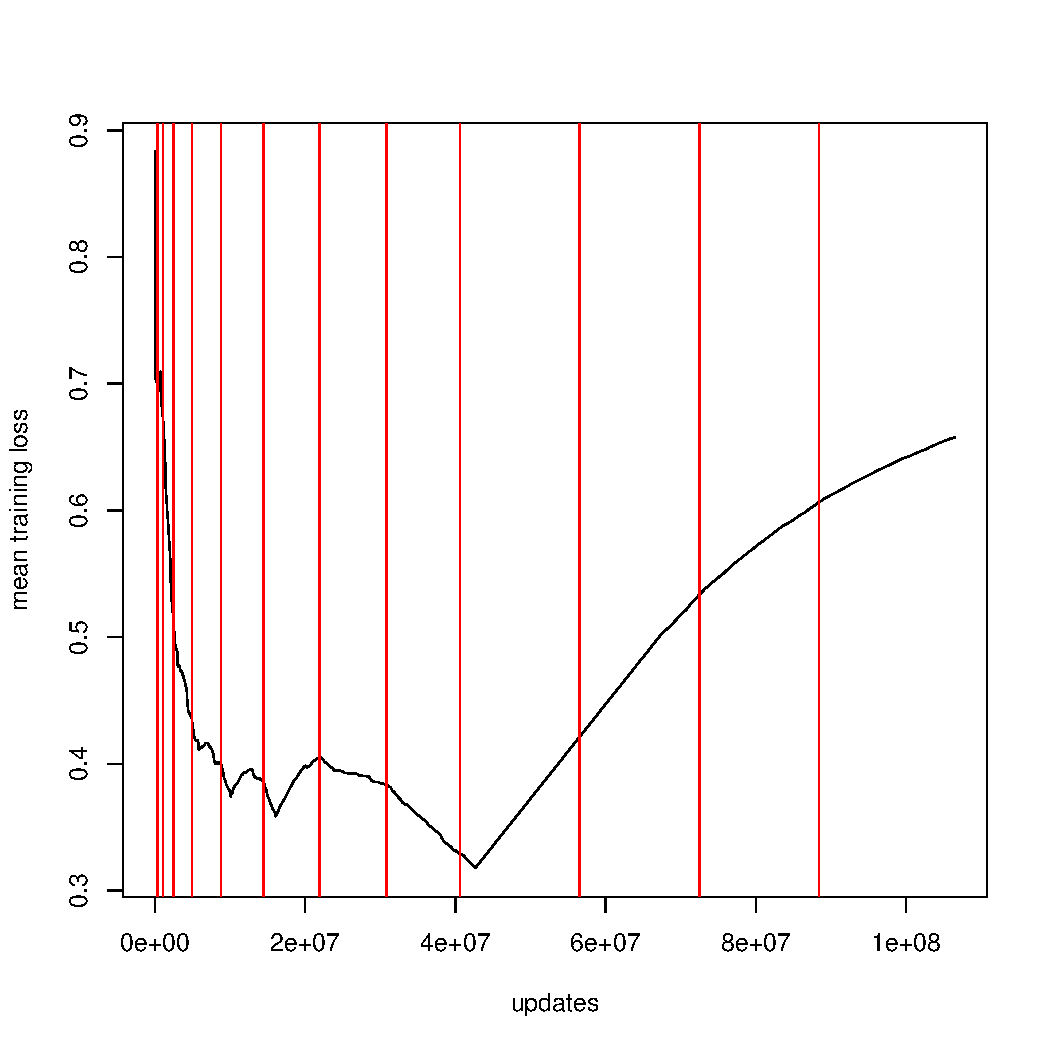
\includegraphics[width=\textwidth]{mean_training_loss}
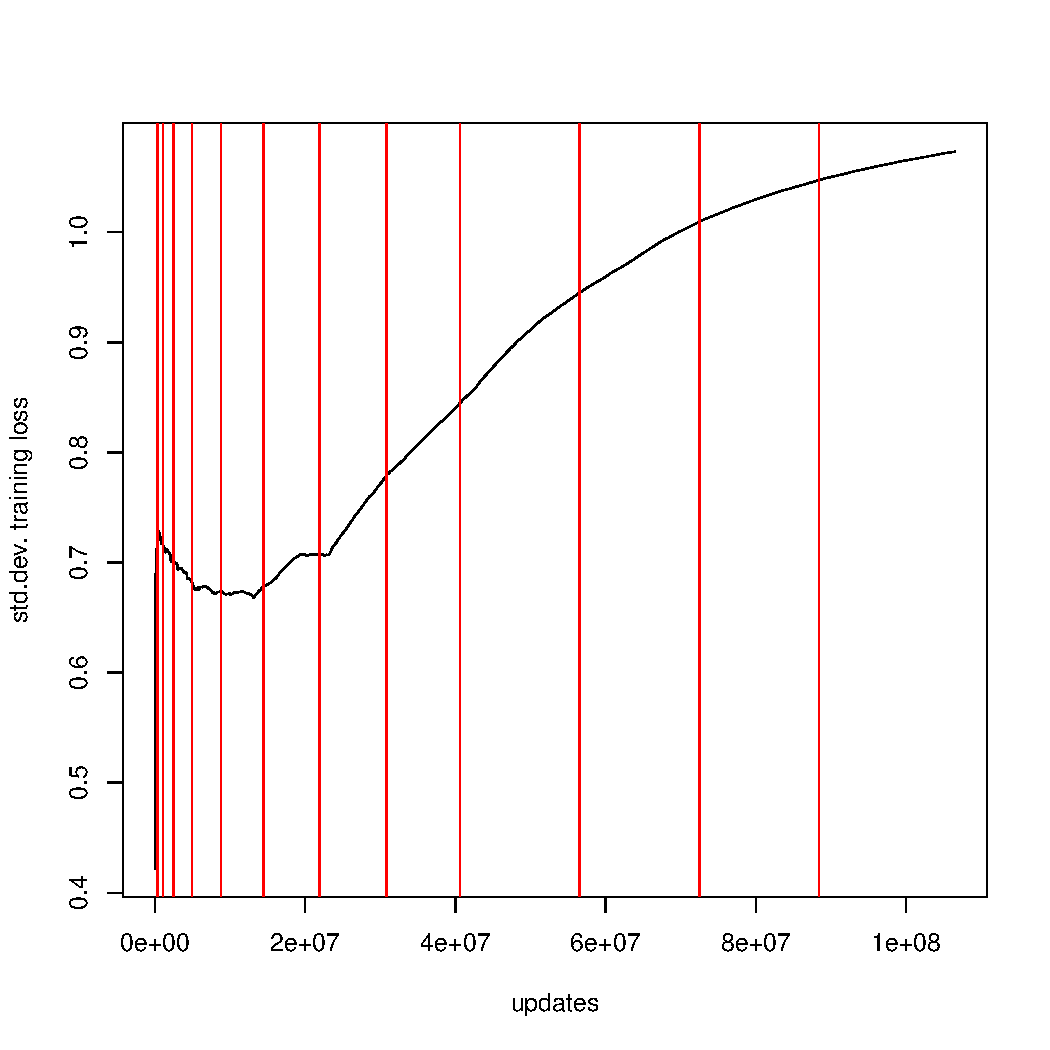
\includegraphics[width=\textwidth]{stddev_training_loss}
\caption{Mean and standard deviation for values of the pairwise ranking cost function.}
\label{fig:training_loss}
\end{figure}

\begin{figure}
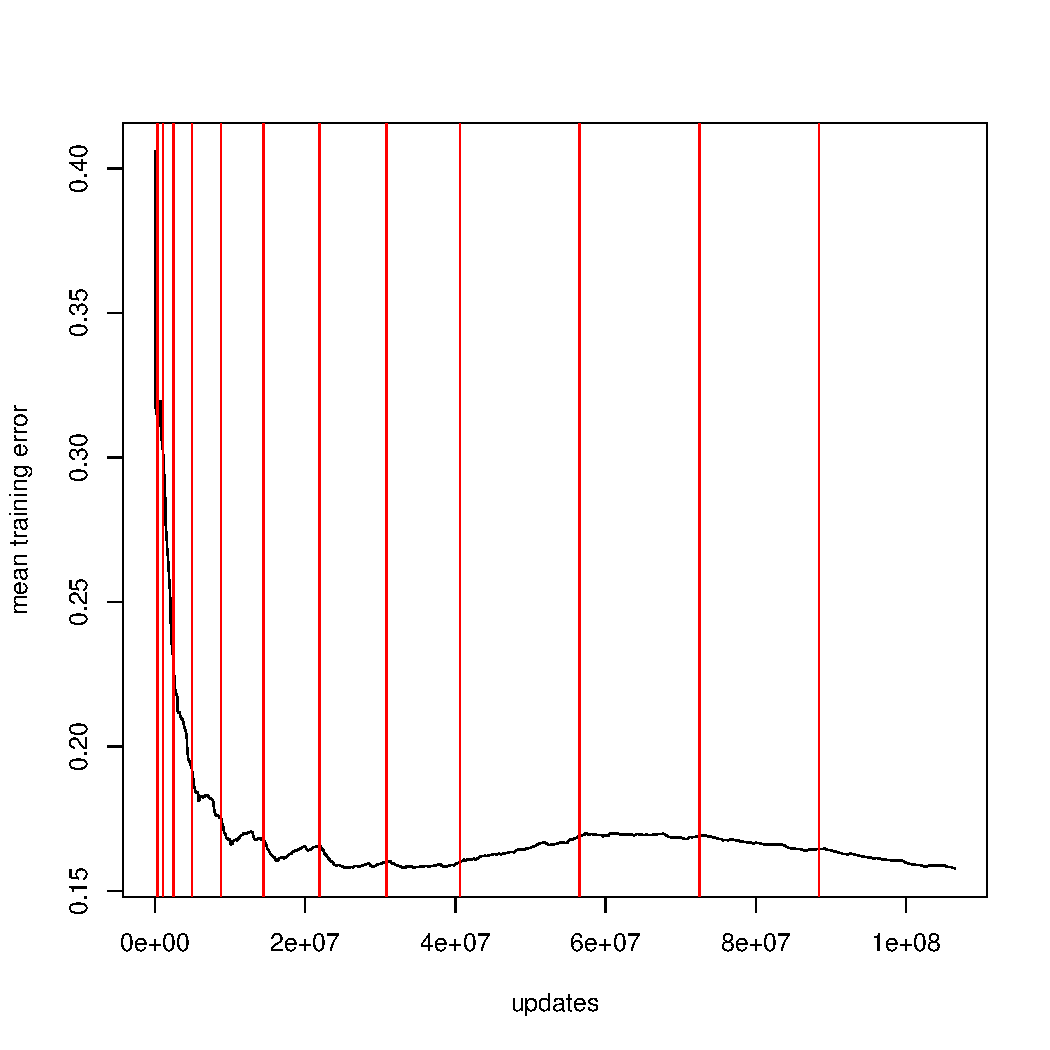
\includegraphics[width=\textwidth]{mean_training_error}
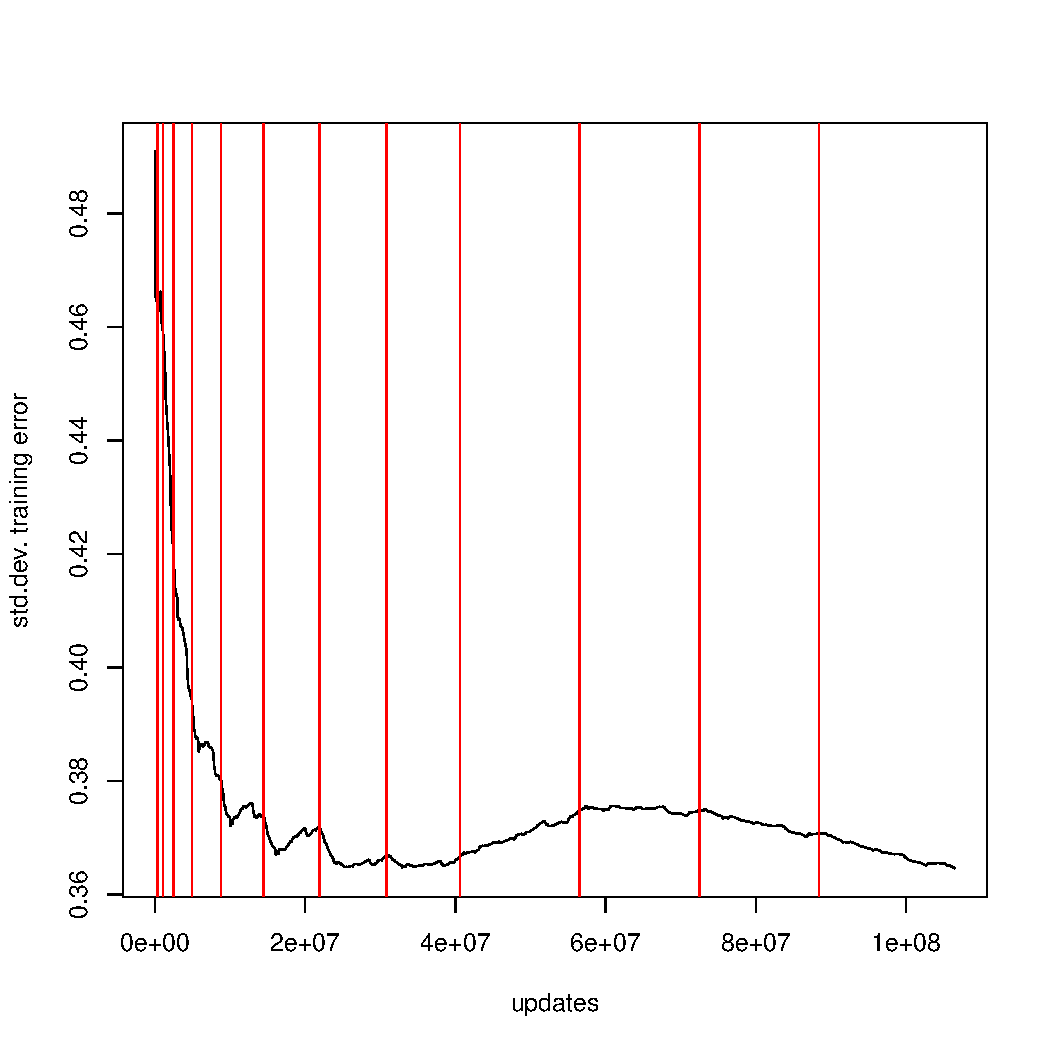
\includegraphics[width=\textwidth]{stddev_training_error}
\caption{Mean and standard deviation of the number of erroneous scores
(i.e. amount of times correct windows were rated lower than corrupted
windows).}
\label{fig:training_error}
\end{figure}

\begin{figure}
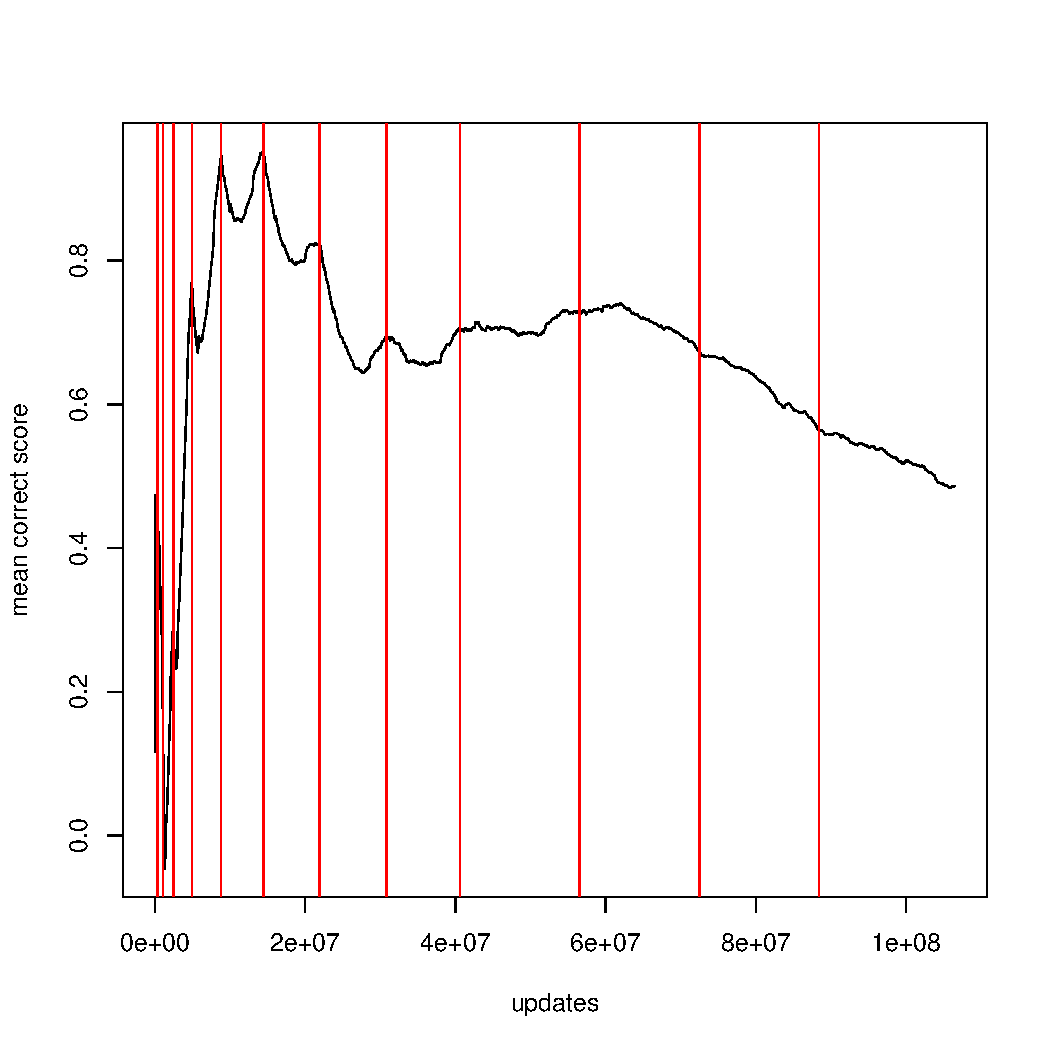
\includegraphics[width=\textwidth]{mean_correct_score}
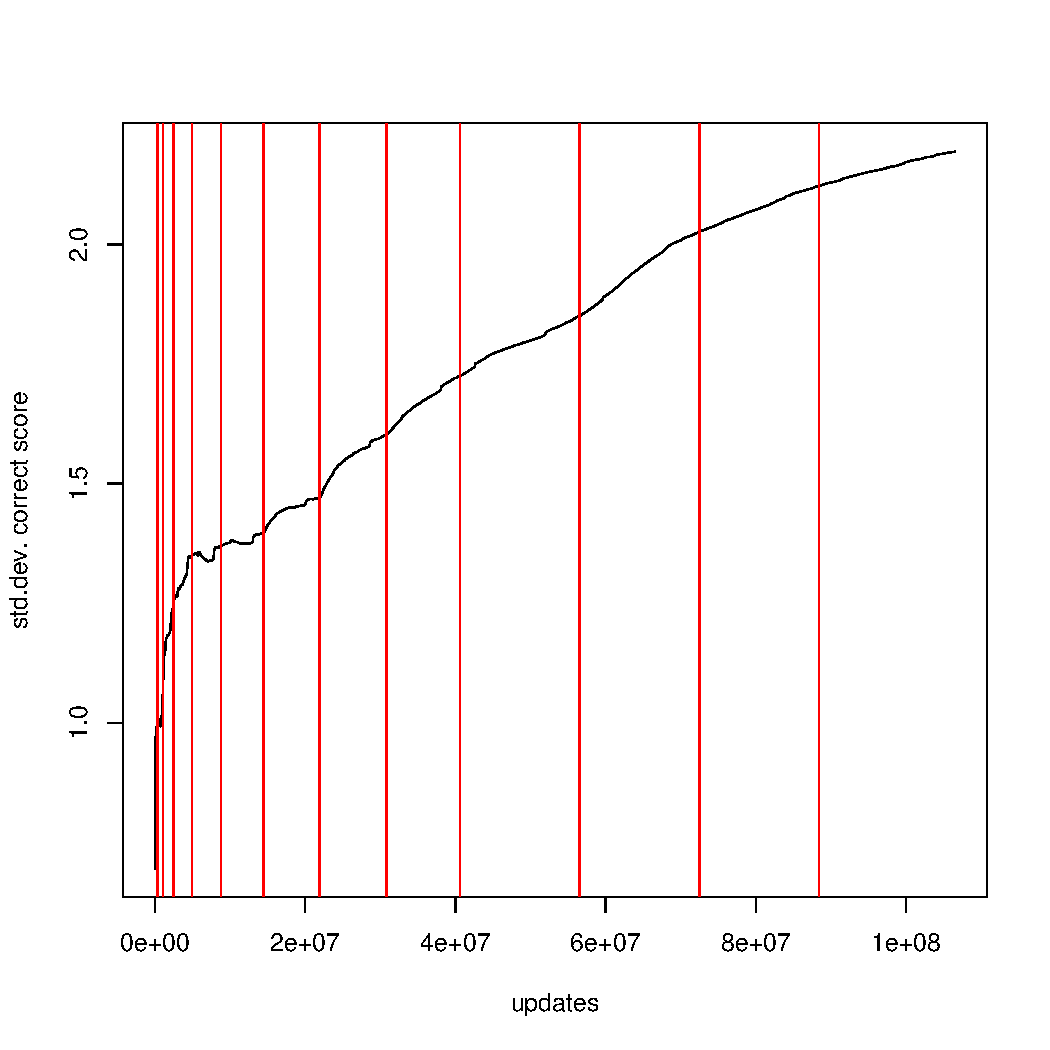
\includegraphics[width=\textwidth]{stddev_correct_score}
\caption{Mean and standard deviation for scores of correct windows.}
\label{fig:correct_score}
\end{figure}

\begin{figure}
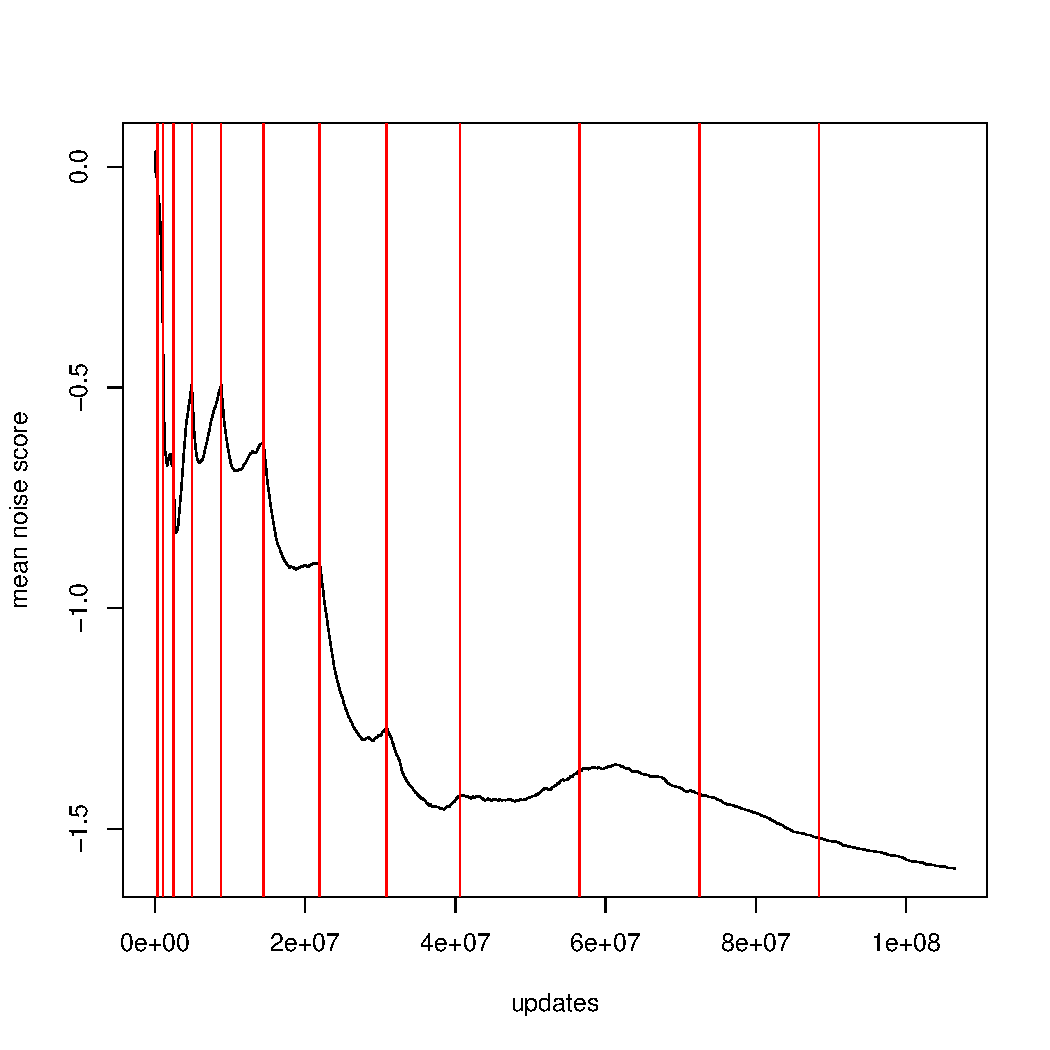
\includegraphics[width=\textwidth]{mean_noise_score}
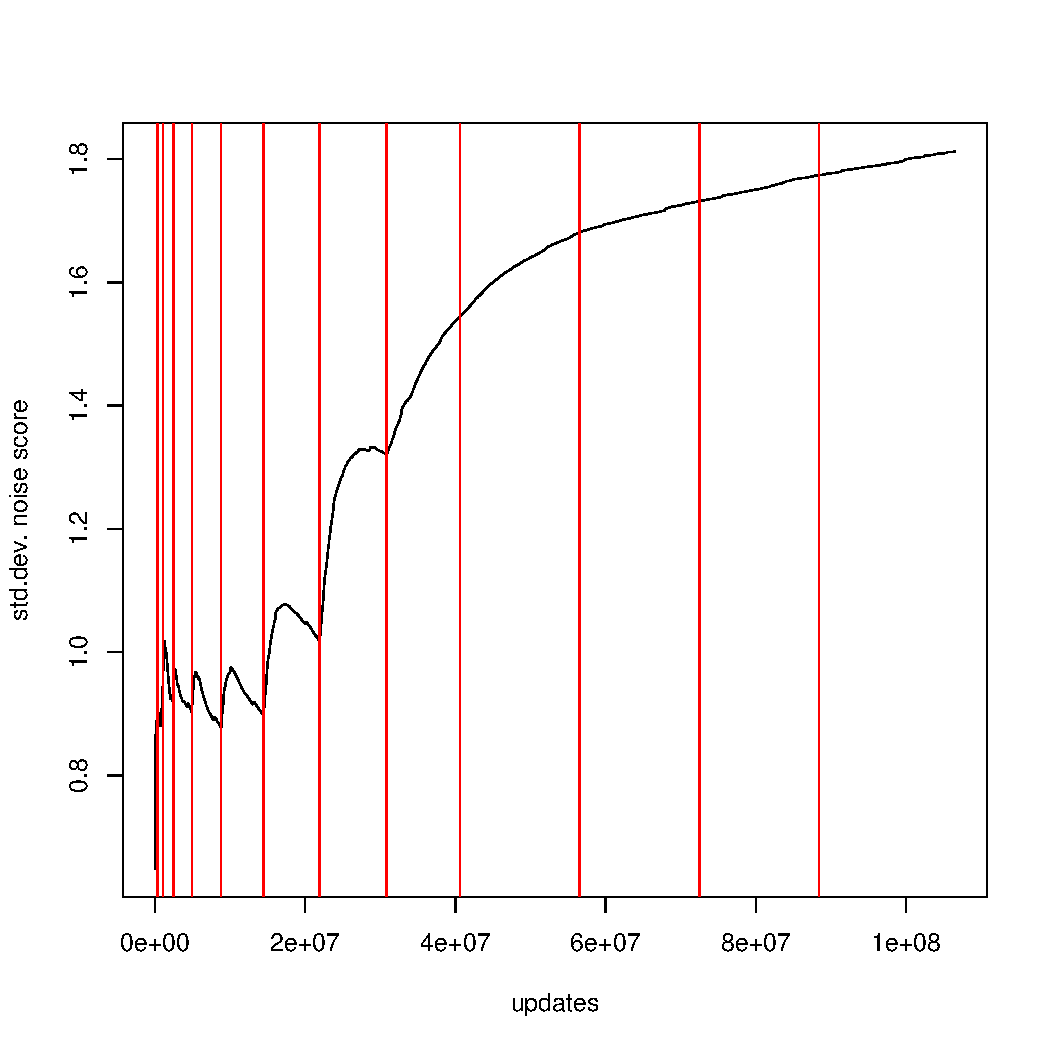
\includegraphics[width=\textwidth]{stddev_noise_score}
\caption{Mean and standard deviation for scores of corrupted windows.}
\label{fig:noise_score}
\end{figure}

\subsection{Supervised model}
\label{sec:supacc}
See \ref{chp:assessment}.